\chapter{PICKING DOS TEMPOS DE TRÂNSITO E MODELAGEM}
\label{cap9}

A estratégia de otimização do modelo de velocidades é baseada no método de empilhamento Elemento de Reflexão Comum (ERC).
Este método é uma alternativa ao empilhamento convencional no domínio do Ponto Médio Comum (PMC), tem como
objetivo a construção da seção empilhada a partir de um conjunto de seções de afastamento constante e
fornecer parâmetros importantes na construção do macro modelo de velocidades \cite{cre}.

Estes parâmetros são o raio de curvatura $R_{NIP}$ e o ângulo de emergência do raio normal $\beta_0$ dados para
uma frente de onda hipotética (Onda PIN) que se origina sobre o refletor em um ponto chamado de Ponto de Incidência Normal
(PIN) \cite{hubral}. Assim, a estratégia de inversão do modelo de velocidades consiste em, a partir dos parâmetros $R_{NIP}$
e $\beta_0$, encontrar o modelo que localiza as fontes pontuais PIN sobre o refletor em profundidade.
A estratégia que iremos utilizar é baseada na NIP tomografia \cite{niptomo} e na Stereo tomografia \cite{stereo}.

\begin{figure}[H]
\caption{Modelo de velocidades de três camadas utilizado para a obtenção da seção
empilhada ERC através do empilhamento ERC.}
\begin{center}
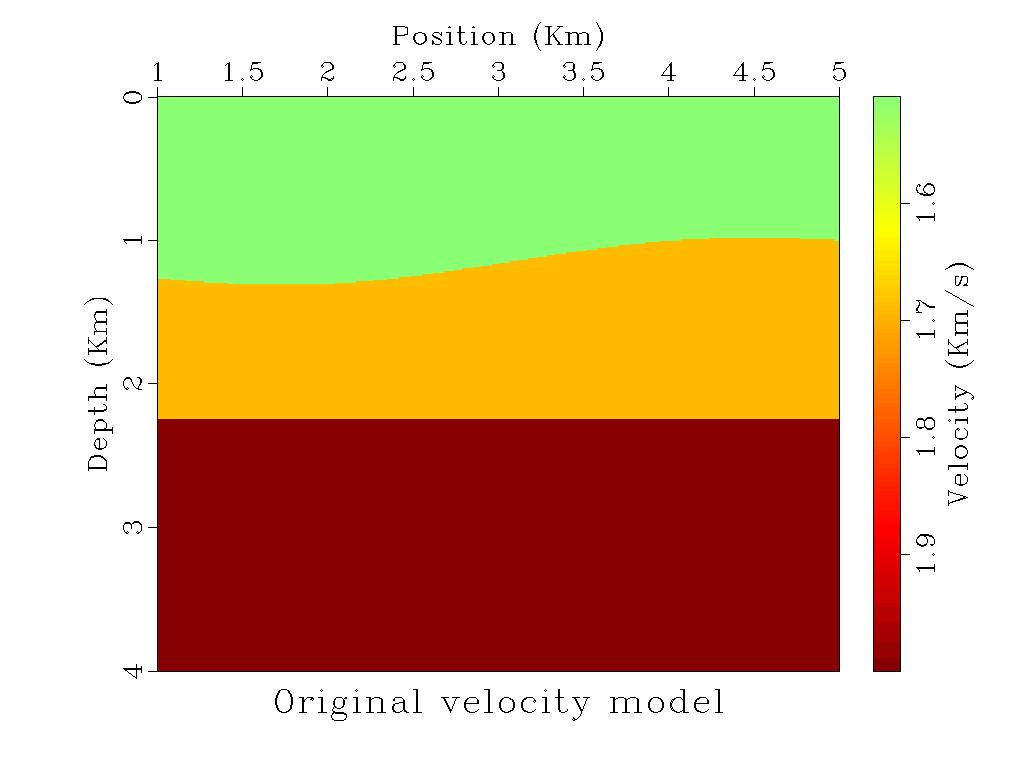
\includegraphics[scale=0.3]{images/mod1.jpeg}
\vspace{-0.3cm}
\end{center}
\begin{center}
 Fonte: Do Autor.
\end{center}
\label{fig:9.1}
\end{figure}

\begin{figure}[H]
\caption{Picking dos tempos de trânsito sobre um refletor da seção empilhada ERC. Os pontos
em amarelo são os pares $t_0$ e $m_0$ escolhidos.}
\begin{center}
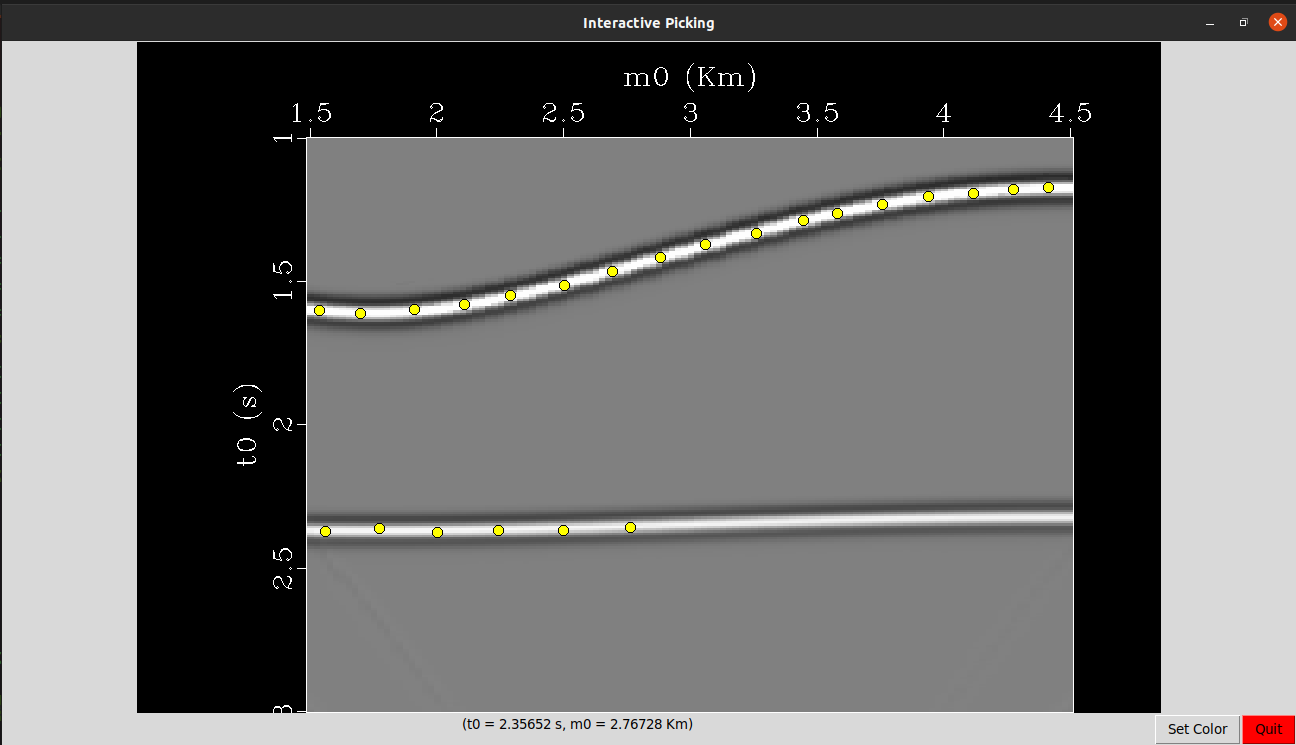
\includegraphics[scale=0.3]{images/picking.png}
\vspace{-0.3cm}
\end{center}
\begin{center}
 Fonte: Do Autor.
\end{center}
\label{fig:9.2}
\end{figure}

\begin{figure}[H]
\caption{Exemplo esquemático do traçamento de raios normais a partir de uma coordenada de um CMP $m_0$
na superfície de aquisição em direção ao modelo em profundidade.
O raio normal (seta) parte da superfície de aquisição com ângulo $\beta_0$ e incide normal
ao refletor no Ponto de Incidência Normal (PIN).}
\begin{center}
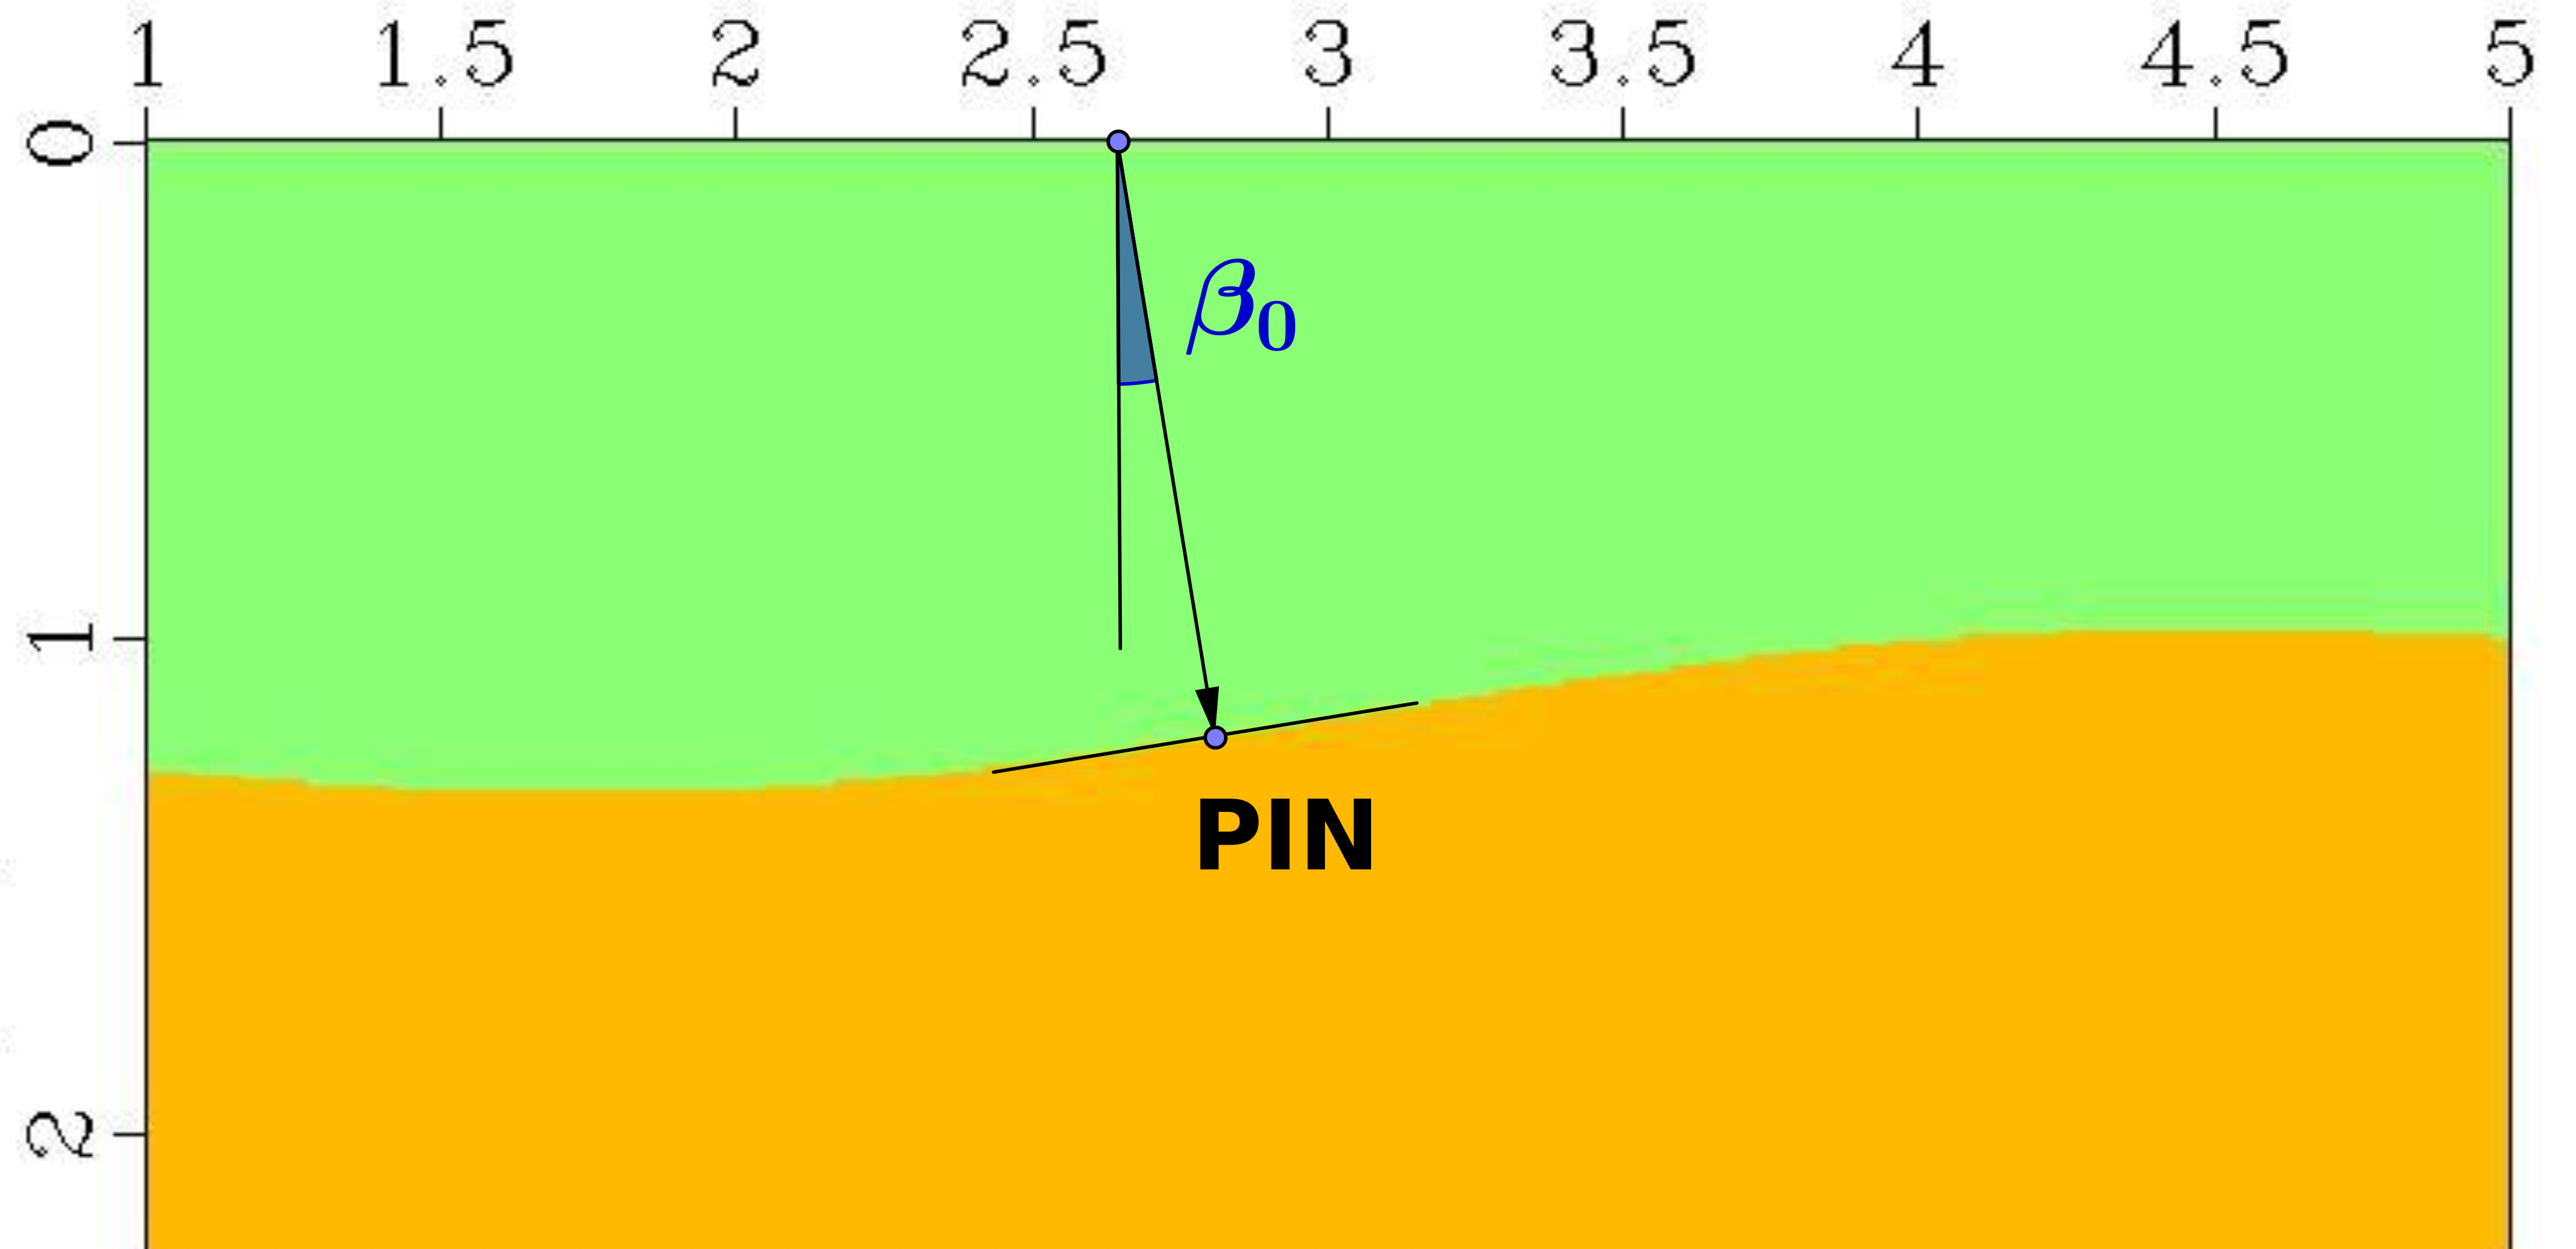
\includegraphics[scale=0.5]{images/modelagem.png}
\vspace{-0.3cm}
\end{center}
\begin{center}
 Fonte: Do Autor.
\end{center}
\label{fig:9.3}
\end{figure}

Para testar a nossa estratégia de inversão obtemos a seção empilhada ERC através do empilhamento ERC
realizado a partir do modelo de velocidades da Figura \ref{fig:9.1},
com três camadas com as velocidades $1.508Km/s$, $1.690Km/s$ e $2.000Km/s$ respectivamente,
utilizando a metodologia de empilhamento ERC descrita no Capítulo 8.
Realizamos o picking interativo dos tempos de trânsito, selecionando manualmente alguns
pontos sobre os refletores na seção empilhada ERC
(Ver Figura \ref{fig:9.2}, pontos em amarelo).
Estes tempos de trânsito selecionados na seção de afastamento nulo (seção empilhada ERC)
são os tempos duplos $t_0$ dos raios normais que partem da coordenada $m_0$
de um PMC na superfície de aquisição e incidem normais ao refletor no ponto PIN (Figura \ref{fig:9.3}).

Os tempos de trânsito $t_0$ escolhidos são utilizados para traçar raios normais
a partir da superfície de aquisição em direção ao modelo de velocidades
em profundidade,
de modo a determinar a possível localização do refletor no modelo
para um determinado modelo de velocidades.
O traçamento continua até que metade do tempo de trânsito $t_0$ seja consumido.
O modelo de velocidades inicial é um modelo de velocidade constante igual à velocidade $v_0$
próxima da superfície de aquisição. O programa para o traçamento de raios foi desenvolvido
utilizando as interfaces da Application Programming Interface (API)
do pacote de processamento sísmico Madagascar \cite{madagascar}
e da construção de uma versão modificada do programa para traçamento de raios 
\textit{sfrays2} que realiza o traçamento cinemático dos raios
através do método Runge-Kutta (Ver Figura \ref{fig:9.4}).

Cada raio normal é iniciado na superfície de aquisição na posição da coordenada $m_0$ e lançado no modelo 
com a direção inicial dada pelo parâmetro $\beta_0$.
O ponto final do raio é a possível localização do refletor em profundidade
e onde será estabelecida a localização das fontes pontuais PIN para o modelo de velocidade
constante. O vetor vagarosidade neste ponto é
normal ao refletor, e com estas informações, o modelo de velocidades inicial é configurado \cite{niptomo}.

\begin{figure}[H]
\caption{Exemplo de traçamento do raio utilizando o programa \textit{sfrays2}
em direção a um modelo de velocidades suavizado.
Este programa está disponível no pacote de processamento sísmico Madagascar e foi
modificado para obter a localização das fontes PIN nos modelos de velocidade deste relatório.}
\begin{center}
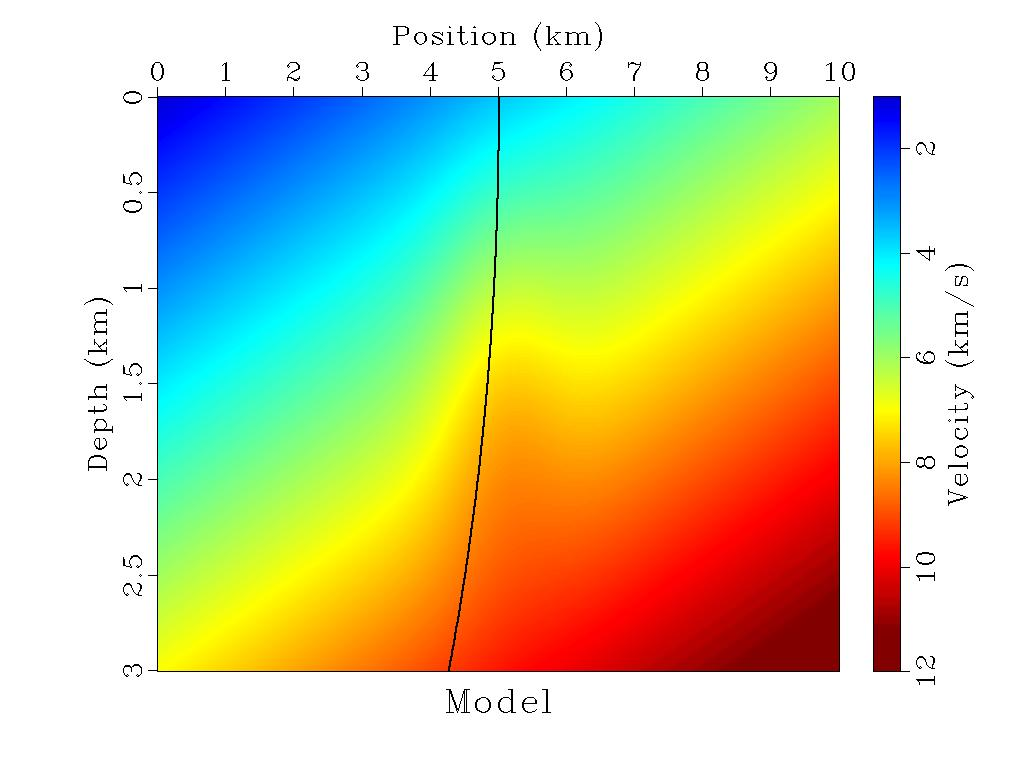
\includegraphics[scale=0.3]{images/raiomodelo.jpg}
\vspace{-0.3cm}
\end{center}
\begin{center}
 Fonte: Do Autor.
\end{center}
\label{fig:9.4}
\end{figure}

Após a determinação das fontes, a modelagem direta é realizada através do traçamento de pares de raios de reflexão
iniciando nas posições das fontes PIN determinadas anteriormente,
simulando uma família ERC de raios de reflexão que atingem a superfície de aquisição
na posição da fonte $x_s$ e do receptor $x_r$.
Este leque de raios é lançado em direção à superfície de aquisição,
os tempos de trânsito dos raios são armazenados \cite{stereo}.

\begin{figure}[H]
\caption{Exemplo esquemático do traçamento de raios a partir do ponto PIN em profundidade.
Os raios são lançados com o mesmo ângulo $\theta_i$ em relação à normal ao refletor no ponto
PIN de modo a simular raios de reflexão de uma família ERC que atingem a superfície de aquisição
na posição da fonte $x_s$ e do receptor $x_r$.}
\begin{center}
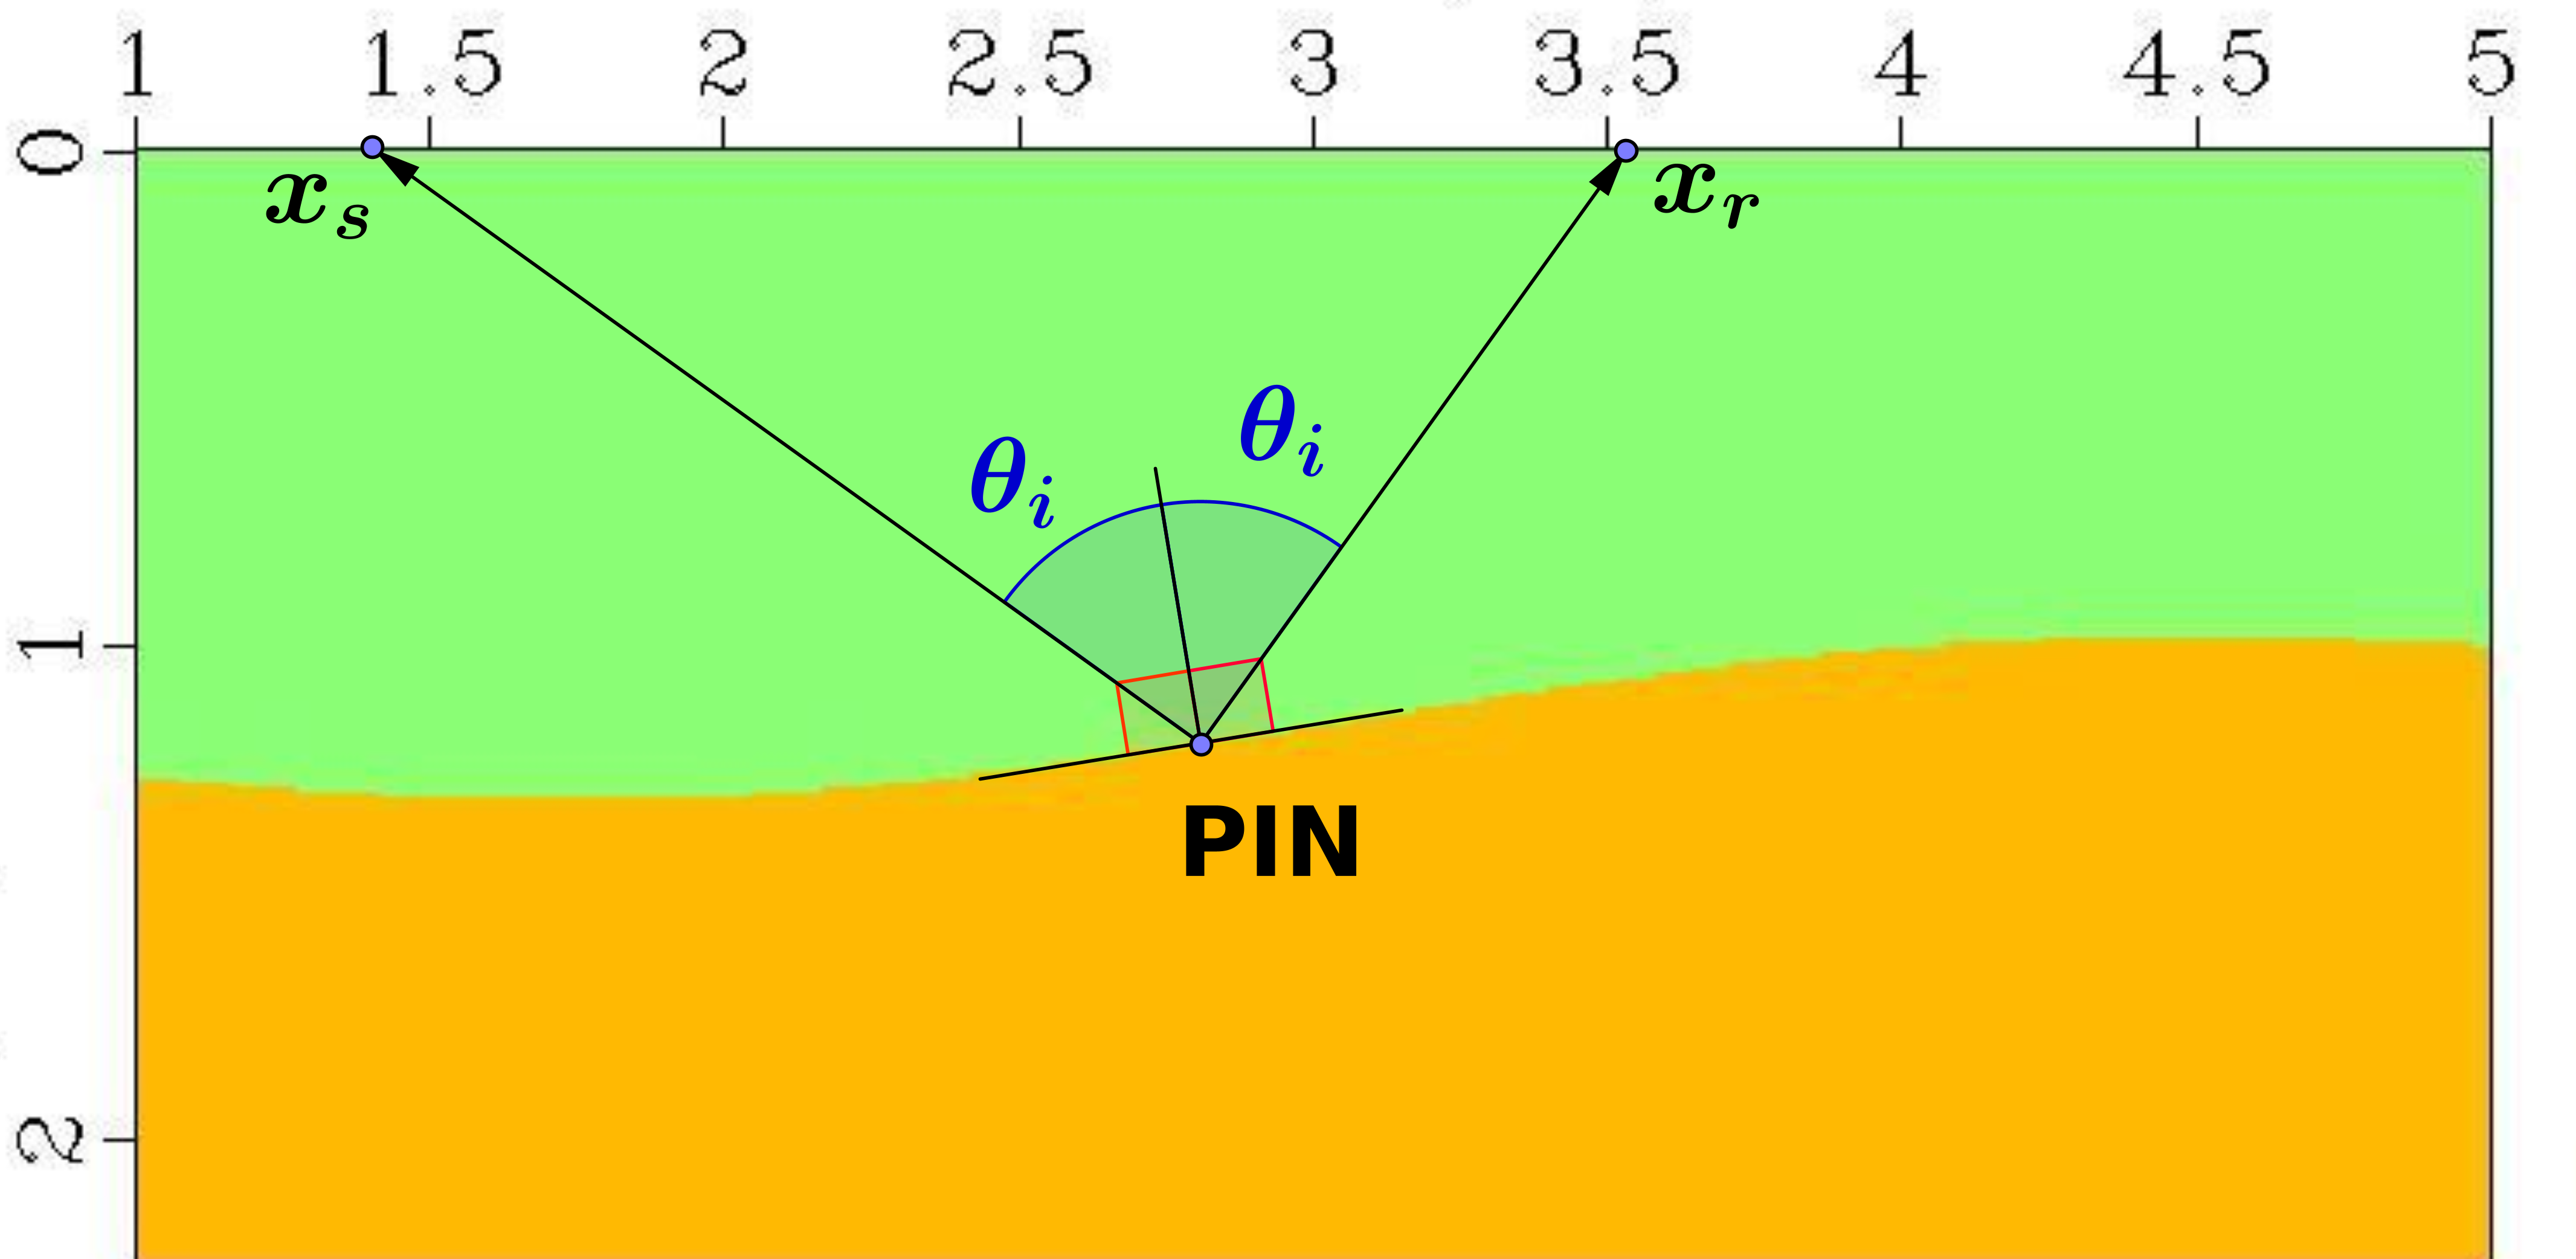
\includegraphics[scale=0.5]{images/modelagem2.png}
\vspace{-0.3cm}
\end{center}
\begin{center}
 Fonte: Do Autor.
\end{center}
\label{fig:9.5}
\end{figure}

Os tempos de trânsito dos raios de reflexão obtidos no traçamento de raios são comparados com os tempos
de trânsito da aproximação de tempo de trânsito ERC a seguir \cite{cre}:

\begin{multline}
\label{eq:9.1}
t(h,m)= \left( \tau_0-\frac{2R_{NIP}}{v_0} \right) 
+\frac{R_{NIP}}{v_0}\sqrt{1-2\alpha(m-m_0+h)+\frac{(m-m_0+h)^2}{R_{NIP}^2}} \\
+\frac{R_{NIP}}{v_0}\sqrt{1+2\alpha(m-m_0-h)+\frac{(m-m_0-h)^2}{R_{NIP}^2}}
\end{multline}

\begin{figure}[H]
\caption{Exemplo de traçamento do raio utilizando o programa \textit{sfrays2}
de um ponto no modelo de velocidades suavizado em direção à superfície de aquisição.
Este programa está disponível no pacote de processamento sísmico Madagascar e foi
modificado para a realização da modelagem direta neste relatório.}
\begin{center}
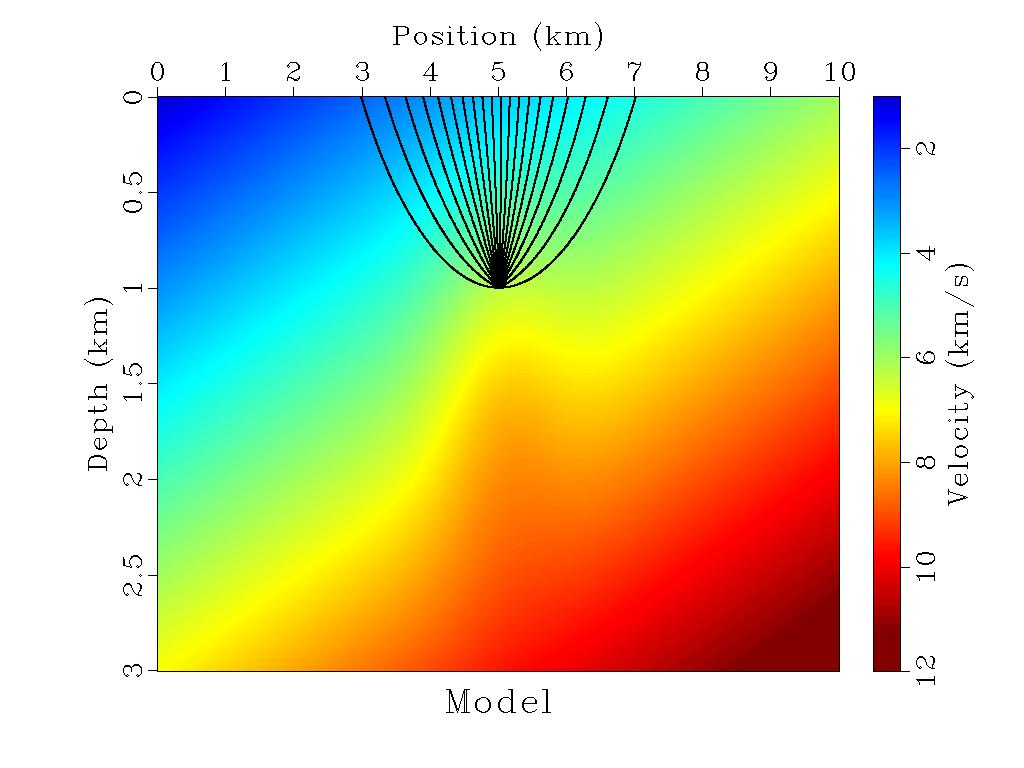
\includegraphics[scale=0.3]{images/raioleque.jpg}
\vspace{-0.3cm}
\end{center}
\begin{center}
 Fonte: Do Autor.
\end{center}
\label{fig:9.6}
\end{figure}

Onde $m$ é a coordenada do PMC, $h$ é a coordenada do afastamento entre fonte e receptor e
$\alpha$ é um parâmetro de assimetria dado em função de $R_{NIP}$ e $\beta_0$.
As diferenças $e_i$ entre os tempos de trânsito do traçamento de raios e dos tempos de trânsito
calculados são somadas segundo a fórmula \cite{stoffa}:

\begin{equation}
\label{eq:9.2}
L_2 = \left[ \sum_{i=1}^{ND} |e_i|^2 \right]^\frac{1}{2}
\end{equation}

As posições $x_s$ e $x_r$ são dadas pelo traçamento de raios armazenando as coordenadas de chegada
na superfície de aquisição dos raios de reflexão simulados na modelagem direta. Estas coordenadas podem
ser transformadas nas coordenadas do afastamento $h$ e PMC $m$ pelas Equações a seguir:

\begin{equation}
\label{eq:9.3}
h = (x_r-x_s)/2
\end{equation}

\begin{equation}
\label{eq:9.4}
m = (x_r+x_s)/2
\end{equation}

Como $\beta_0$, $R_{NIP}$ são parâmetros conhecidos para cada raio normal e obtidos do empilhamento
ERC e $v_0$ é a velocidade próximo da superfície de aquisição, também conhecida, podemos calcular o
tempo de trânsito esperado com a Equação \ref{eq:9.1} e comparar com o tempo de trânsito do raio de
reflexão simulado
dado pela soma dos tempos do raio que sai do ponto PIN e chega em $x_s$ ($\Delta \tau_s$)
e do raio
que sai do ponto PIN e chega em $x_r$ ($\Delta \tau_r$), esta diferença deve ser mínima para o modelo de velocidades
correto (ver Figura \ref{fig:9.5}). A soma dos tempos de trânsito obtidas com o
traçamento de raios é dada a seguir:

\begin{equation}
\label{eq:9.5}
\tau(h,m) = \Delta \tau_s + \Delta \tau_r
\end{equation}

Assim, a diferença $e_i$ e a norma dois $L_2$ da Equação \ref{eq:9.2} podem ser estabelecidas como:

\begin{equation}
\label{eq:9.6}
L_2 = \left[ \sum_{i=1}^{ND} |e_i|^2 \right]^\frac{1}{2}
= \left[ \sum_{i=1}^{ND} |\tau(h,m)-t(h,m)|^2 \right]^\frac{1}{2}
\end{equation}

Esta estratégia de modelagem direta será utilizada nas etapas de inversão do modelos de velocidades nos
próximos capítulos. A norma dois das diferenças nos tempos de trânsito (Equação \ref{eq:9.2})
será utilizada como critério de
convergência do modelo de velocidades: O modelo de velocidades otimizado deverá produzir
o valor mínimo das diferenças entre os tempos de trânsito obtidos com o traçamento de raios
e calculados com a fórmula do ERC (Equação \ref{eq:9.1}). Assim, a estratégia de inversão consiste em
encontrar o modelo de velocidades que produz o mínimo global da Equação \ref{eq:9.2}.

